\documentclass[handout]{beamer}
\usepackage[utf8]{inputenc}
\usepackage{amsmath, pdfpages, pdflscape, lscape, color, listings, hyperref, amssymb, graphicx,textcomp,varioref, afterpage, subcaption, float, bm, tikz, multicol} 

\global
\newcommand{\Fig}[1]{Figure \ref{#1}}
\newcommand{\fig}[1]{figure \ref{#1}}
\newcommand{\tab}[1]{table \ref{#1}}
\newcommand{\eq}[1]{equation \ref{#1}}
\newcommand{\Eq}[1]{Equation \ref{#1}}
\newcommand{\alg}[1]{algorithm \ref{#1}}
\newcommand{\Alg}[1]{Algorithm \ref{#1}}
\newcommand{\chp}[1]{chapter  \ref{#1}}
\newcommand{\Chp}[1]{Chapter  \ref{#1}}
\newcommand{\e}[1]{\cdot 10^{#1}}
\newcommand{\h}{\hbar}
\newcommand{\der}[2]{\frac{\partial #1}{\partial #2}}
\newcommand{\dder}[2]{\frac{\partial^2 #1}{\partial #2^2}}
\newcommand{\p}{\boldsymbol{P}}
\newcommand{\q}{\boldsymbol{q}}
\newcommand{\norm}[1]{\left\lVert#1\right\rVert}
\newcommand{\coef}[2]{\frac{\langle #1,#2\rangle_Q}{\norm{#2}^}}


\newenvironment{test}[1]
{
 \usebackgroundtemplate{}
 \color{gray!30!black}
   \begin{tikzpicture}[remember picture, overlay]
     \node[anchor = center, opacity=.25] (image) at (current page.center) {
\includegraphics[scale=0.25]{chaospy_logo.jpg}};
   \end{tikzpicture}
 \begin{frame}[fragile,enviroment=chaospy]
   
}
{
 \end{frame}
}

\lstset{
escapeinside=||
}


\newenvironment{chaospy}[1]
{\color{gray!30!black}
     \color{gray!30!black}
     \usebackgroundtemplate{
   \begin{tikzpicture}[remember picture, overlay]
     \node[anchor = center, opacity=.25] (image) at (current page.center) {
\includegraphics[scale=0.25]{chaospy_logo.jpg}};
   \end{tikzpicture}}
     \begin{frame}[fragile,environment=chaospy]
    \frametitle{{#1}}}
{\end{frame}}


\definecolor{keywords}{RGB}{255,0,90}
\definecolor{comments}{RGB}{0,0,113}
\definecolor{red}{RGB}{160,0,0}
\definecolor{green}{RGB}{0,150,0}
 
\usetheme{kalkulo}

\graphicspath{{./figures/}}


\title{Polynomial chaos expansions: Exercises}
\author{Jonathan Feinberg and Simen Tennøe}


\begin{document}


\begin{frame}
  \maketitle
\end{frame}


% \begin{frame}
% \frametitle{Traveling with constant velocity, a simple problem}
%    \begin{alert}{Interactive session:}
% \href{http://10.50.3.247:8888/}{http://10.50.3.247:8888/}
%   \end{alert}
%  
%    
%     \begin{alert}{Example code:}
% \href{https://github.com/hplgit/chaospy/blob/master/example2.py}{https://github.com/hplgit/chaospy/blob/master/example2.py}\newline
%   \end{alert}  
%  
%   
%  Distance when traveling at constant velocity is
% \[s(t) = vt\]
% \pause
% where the velocity is measured to
% \[v \sim \text{Normal(5, 1)}\]
% \pause
% \begin{alert}{Task:}
%  Find the expectation value and variance in the time interval $t=[0,10]$  and plot them, use Gaussian Quadrature.
% \end{alert}

% \end{frame}

\begin{frame}
\frametitle{Traveling with constant acceleration}
\scriptsize
%    \begin{alert}{Interactive session:}
% \href{http://10.50.3.247:8888/}{http://10.50.3.247:8888/}
%   \end{alert}
%   
    \begin{alert}{Example code:}
\href{https://github.com/hplgit/chaospy/blob/master/example2.py}{https://github.com/hplgit/chaospy/blob/master/example2.py}\newline
  \end{alert}  
 


 Distance when traveling with constant acceleration is
 \[s(t) = v_0t + \frac{1}{2}at^2\]
\pause
The initial velocity and acceleration is measured to
\[v_0 \sim \text{Uniform(1, 2)} \qquad a \sim \text{Beta(2, 2)}\]
\pause
\begin{alert}{Task:}
Find the expectation value and variance in the time interval $t=[0,10]$  and plot them. Use:
\begin{itemize}
    \item Classical Monte Carlo integration.
    \item Quasi-Monte Carlo using \underline{S}obol sequence.
    \item Pseudo-spectral projection with full tensor grid \underline{G}aussian quadrature.
    \item Pseudo-spectral projection with \underline{C}lenshaw-Curtis and Smolyak sparse grid.
    \item Point collocation with random samples and least squares
        minimization.
    \item Point collocation with Ha\underline{m}mersley samples and \underline{T}ikhonov regularization.
\end{itemize}
\end{alert}
\end{frame}

\begin{frame}{A Monte Carlo solution gives}
 \begin{figure}
  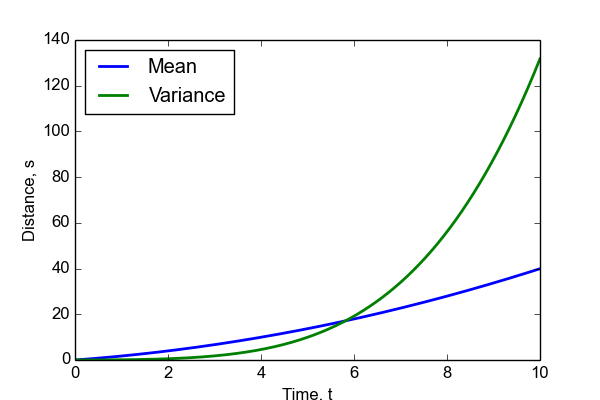
\includegraphics[width=0.85\textwidth]{solution2.png}
 \end{figure}

\end{frame}


\begin{frame}
\frametitle{A different differential equation}
%    \begin{alert}{Interactive session:}
% \href{http://10.50.3.247:8888/}{http://10.50.3.247:8888/}
%   \end{alert}
  
   \begin{alert}{Example code:}
\href{https://github.com/hplgit/chaospy/blob/master/example3.py}{https://github.com/hplgit/chaospy/blob/master/example3.py}\newline
  \end{alert}  
  
We have the differential equation 
\[\frac{d u(x)}{dx} = u(x) + a \qquad u(0) = I,\]
where a and I is uncertain and given by
\[a\sim \text{Normal(4, 1)}\qquad I\sim \text{Uniform(2, 6)}\]
\begin{alert}{Task:}
Find the expectation value and variance in the time interval $t=[0,1]$  and plot them. Use:
\begin{itemize}
 \item A pseudo spectral method with a Rosenblat transformation, map against a Normal(0, 1) and Uniform(-1, 1) distribution.
 \item The intrusive Galerkin method.
\end{itemize}

\end{alert}
\end{frame}

\begin{frame}{A Monte Carlo solution gives}
 \begin{figure}
  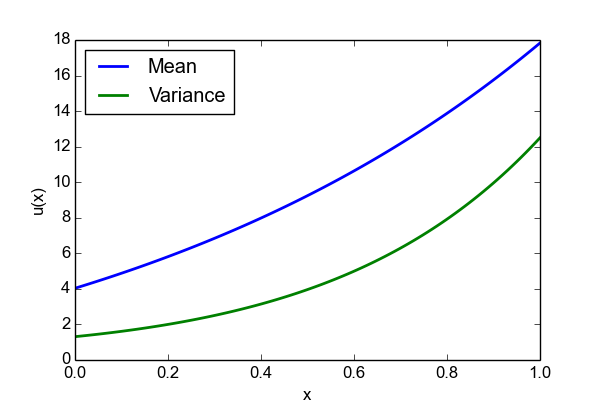
\includegraphics[width=0.85\textwidth]{solution8mc.png}
 \end{figure}

\end{frame}


% \begin{frame}
% \frametitle{Traveling with constant acceleration}
% \scriptsize
%  Distance when traveling with constant acceleration is
%  \[s(t) = v_0t + \frac{1}{2}at^2\]
% \pause
% The initial velocity and acceleration is measured to
% \[v_0 \sim \text{Uniform(1, 2)} \qquad a \sim \text{Beta(2, 2)}\]
% \pause
% \begin{alert}{Task:}
% Find the expectation value and variance in the time interval $t=[0,10]$  and plot them. 
% \begin{itemize}
%     \item 
% \end{itemize}
% \end{alert}
% \end{frame}



\end{document}
